\section{Measurements}

This is the main bulk of our paper, and we discuss the method with which we approached this problem,
the strategies we implemented and our results.

\subsection{Methodology}

To model this system, we constructed a simulation framework in C++.
This framework translated and encoded our assumptions as best as we could.
It used basic C++ polymorphism to capture the ideas of Metrics, Strategies and Simulations and then
write them to files.\\
\\
A more complete description of its inner workings is described in Appendix \ref{simframe}.
We will review the strengths and weaknesses of this approach in the analysis, found in Section
\ref{analysis}.

\subsection{Strategies}

We will look at three strategies for defect detection and fixing.
In particular, we will also vary these strategies according to some metrics, and say that a
simulation is finished according to the results of another metric.\\
\\
Firstly, we make the following assumptions about a strategy for defect detection and fixing.
\begin{itemize}
	\item a strategy is stateful in the sense that it remembers previous defect detections and makes
judgements on whether to finish or to reallocate resources based on that state
	\item since it is stateful, strategies are inherently measuring and then making decisions based on
a metric and it is thus reasonable to assume that strategies require metrics to function well
	\item a strategy should at all times allocate all engineers to some task
	\item a strategy will reorder the defect queue based upon some criterion of the strategy
	\item strategies will favour defects found earlier over defects found later
	\item strategies will stop when a system is estimated to have too few defects remaining or the
number of defects has stabilised to the point that it is a waste of resources to continue testing
\end{itemize}

We will look at the following three strategies
\begin{enumerate}
	\item first-in-first-out (FIFO) --- earlier defects are favoured over later defects, but there is no
ordering between these defects.\\
	As an example, all defects in week 1 will be placed ahead in the queue compared to defects found
in week 2, but the hard, easy, major and minor defects of week 1 have no inherent ordering over each
other
	\item easy first --- extends the FIFO strategy, by now placing an ordering that we prefer easy
defects to hard defects, and then major defects to minor defects.\\
	This means that, in order, we prefer easy major defects, then easy minor defects, then hard major
defects, and lastly hard minor defects.\\
	\item major first --- extends the FIFO strategy, by now placing an ordering that we prefer major 
defects to minor defects, and then easy defects to hard defects.\\
	This means that, in order, we prefer easy major defects, then hard major defects, then easy minor 
defects, and lastly hard minor defects.\\
\end{enumerate}

Our variations on these strategies will be simple resource reallocations, based on either internal
or external pressure.
\begin{itemize}
	\item no variation --- the strategy runs as prescribed and no resource changes occur
	\item external pressure --- the client is being heavily affected by the defects, so the tester is
temporarily reallocated to defect fixing
	\item internal pressure --- upper-level management is unimpressed by the size of the defect queue,
so a tester is temporarily reallocated to defect fixing
\end{itemize}

The actual, well-defined points for when management or a client becomes dissatisfied are somewhat
arbitrarily chosen.
We will expand upon this more within the experiments section, and our later analysis.
We feel that this arbitrariness is a good reflection of real life, however.

Other strategies that we could look at, but will discard are
\begin{itemize}
	\item solve the defects in a random order --- this is illogical, and as our models are supposed to
somewhat reflect real life processes, why should we do something that is entirely contrived and has
no basis in the real world whatsoever?
	\item solve te hard defects first --- this has the least gains for our internal metrics, and a greedy approach dictates
that this is the least efficient use of our time.
	Why solve defects that take more time and are less impactful for the user (and also give us bad
performance overall) when we can pick solve easier problems?
	\item solve minor defects first -- again this has few gains, from the user point of view, since
high impact problems that are really affecting productivity are being ignored.
	If this leads to client dissatisfaction, then why use this strategy?
	Indeed, client-driven engineering suggests that this is the worst kind of strategy to use (see
\FIXME and \FIXME for more details on client-driven engineering and effects of client
dissatisfaction)
\end{itemize}

\subsection{Experiments}

We display the results of our experiments in graphical form, and finally make comments and tabulate
which strategies showed the most promising results.

\subsubsection{No change of resources}

We first begin by looking at the external metrics.
This governs what the client (might!) be thinking about our project and the strategies we have used.

\begin{figure}[ht!]
	\centering
	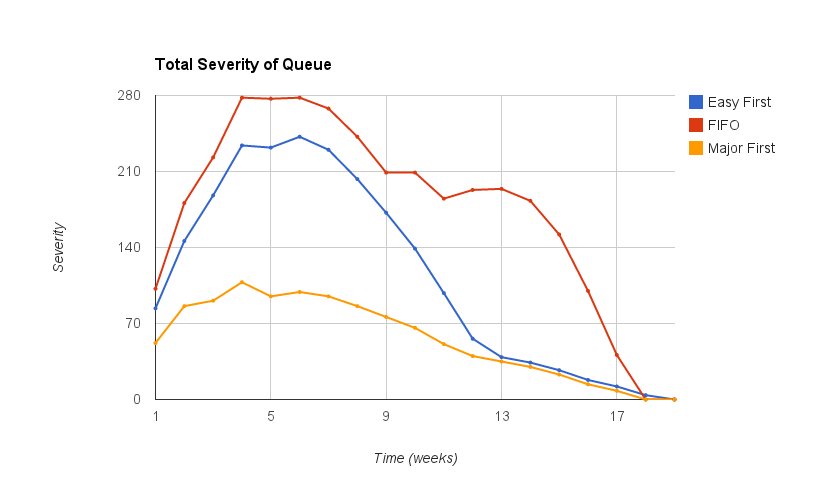
\includegraphics[scale=0.5]{graphs/QueueImpact.png}
	\caption{The severity of the defects yet to be fixed is shown here.
Of note is that defects perhaps should be more impactful the longer they are left in the queue ---
but are we then measuring reputation, money or productivity?
Beyond this, it is quite clear that at this stage fixing major defects first is a good strategy to
take, as it consistently keeps the queue impact low by fixing lots of major defects.} 
	\label{qimpact}
\end{figure}

It is clear that fixing major defects is the best choice according to this metric.
What about the average time of major defects in the queue?
This gives us an idea of how long users have been waiting for a fix to a critical error.

\begin{figure}[ht!]
	\centering
	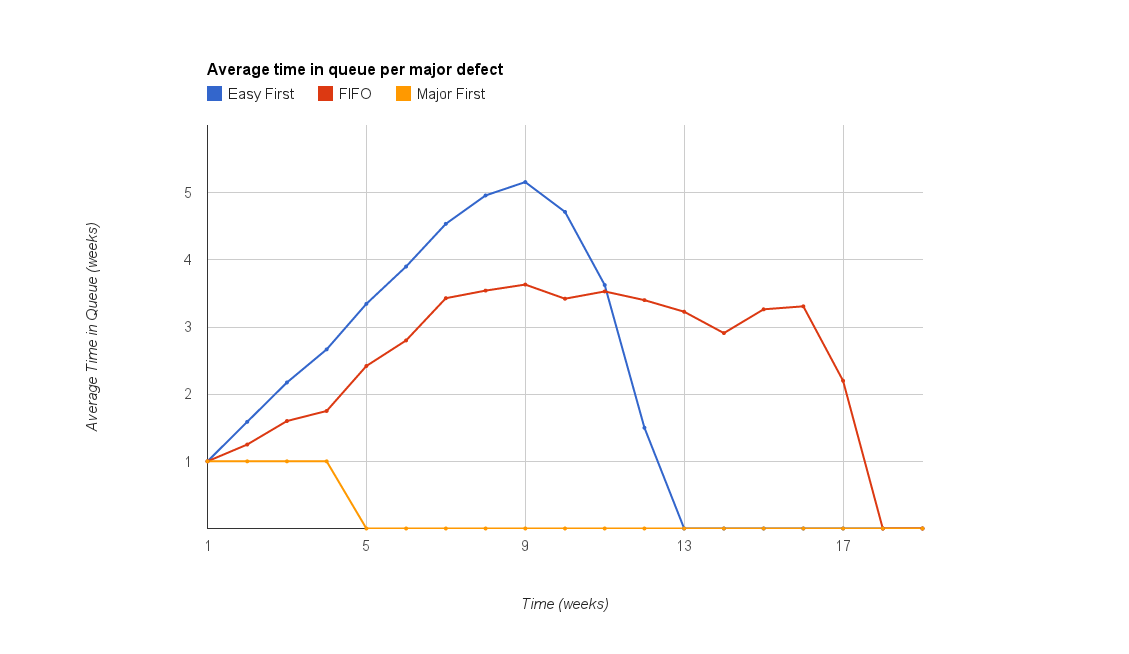
\includegraphics[scale=0.45]{graphs/avgMajorQueueTime.png}
	\caption{High prioritisation of major defects is very helpful here!
	We see that major defects are being fixed almost as they come arrive in the major strategy, whilst
the FIFO and easy-first strategies allow the time in queue to blow up to high values.} 
	\label{avgmajqtime}
\end{figure}

From Figure \ref{avgmajqtime} it is clear that fixing major defects is the best choice to have a
high performance for average major queue time.
This is inherently due to the focus on major defects and giving the customer what they are
interested in (or so we presume).\\
\\
Next, we briefly examine the find-versus-fixed ratio for major defects.

\pagebreak

\begin{figure}[ht!]
	\centering
	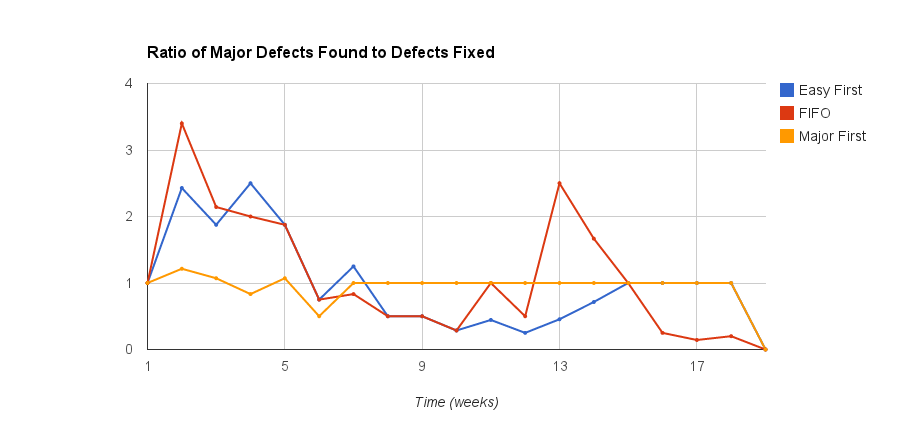
\includegraphics[scale=0.45]{graphs/MajRatioFF.png}
	\caption{High prioritisation of major defects is very helpful here!
	We see that major defects are being fixed almost as they come arrive in the major strategy, whilst
the FIFO and easy-first strategies allow the time in queue to blow up to high values.} 
	\label{majratioff}
\end{figure}

Again we see that the optimal strategy for this metric is to fix major defects first --- not very
surprising!
But it is interesting to note that here, the differences are not so great --- especially towards the
end, the major-fixes-first are either on par or even suboptimal compared to the other two
strategies.\\
\\
Finally in Figure \ref{estremmajdef}, we examine the estimation of how many major defects remain in the system.

\pagebreak

\begin{figure}[ht!]
	\centering
	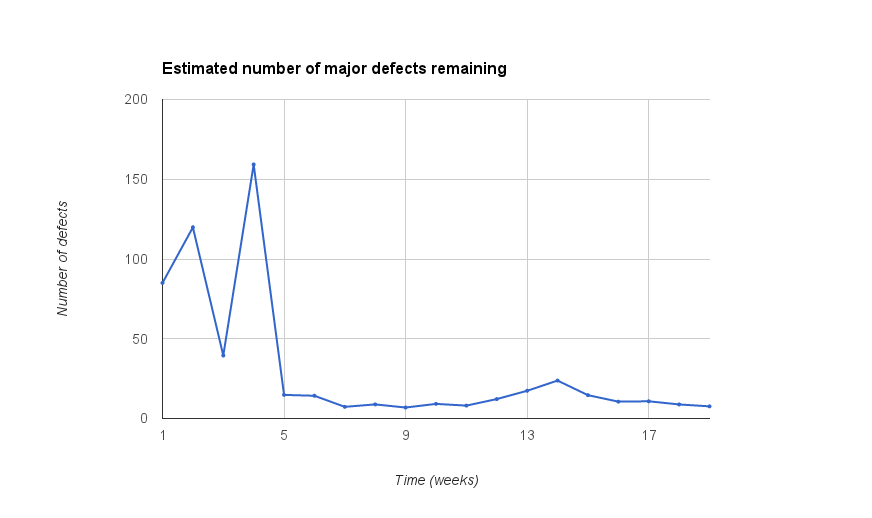
\includegraphics[scale=0.5]{graphs/EstRemMajDef.png}
	\caption{Since each defect has the same detection policies, each of them had the same curve and
there is no ``better" detection here.} 
	\label{estremmajdef}
\end{figure}

It is clear that towards the end of the process there are very few major defects remaining.
But why stop there?\\
\\
To answer this question, we now show the results of our internal metrics.
We begin with the metric ``how many defects do we estimate remain in our system?"

\pagebreak

\begin{figure}[ht!]
	\centering
	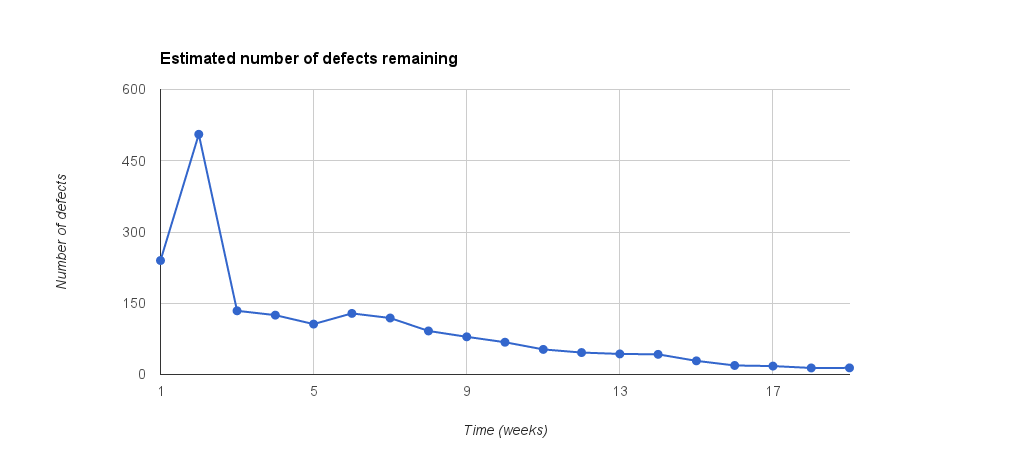
\includegraphics[scale=0.45]{graphs/EstRemDefs.png}
	\caption{Notice how few defects there are towards the end. This is part of the criteria for
stopping a simulation, and the strategy decided that further testing was a waste of resources due to
the estimate saying that the defect counting had stabilised.} 
	\label{estremdefs}
\end{figure}

Again, the system stability and low number of estimated defects towards the end of the development
process is an indicator as to why a project manager would say the project is completed.
But how good are the strategies at keeping the number of defects that need to be fixed low?

\pagebreak

\begin{figure}[ht!]
	\centering
	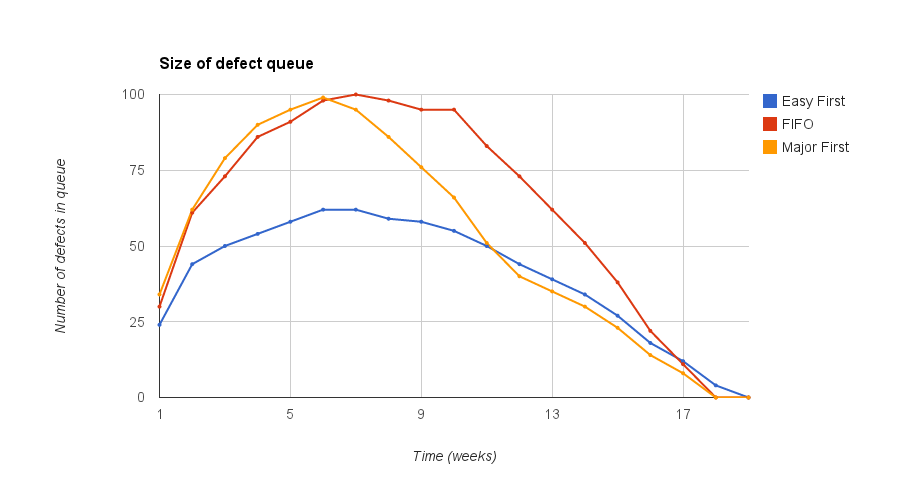
\includegraphics[scale=0.45]{graphs/QueueSz.png}
	\caption{The size of our defects-to-fix queue. The seemingly optimal choice is to use the easy
strategy.} 
	\label{qsz}
\end{figure}

Figure \ref{qsz} gives what would be the self-evident result --- that prioritising easy defects
yields the best rewards.
This is simply because taking easy defects first results in the highest number of defects being
fixed and the queue size shrinking fastest.\\
\\
We would expect something similar to occur when looking at the average time a defect spends in a
queue, wouldn't we?

\pagebreak

\begin{figure}[ht!]
	\centering
	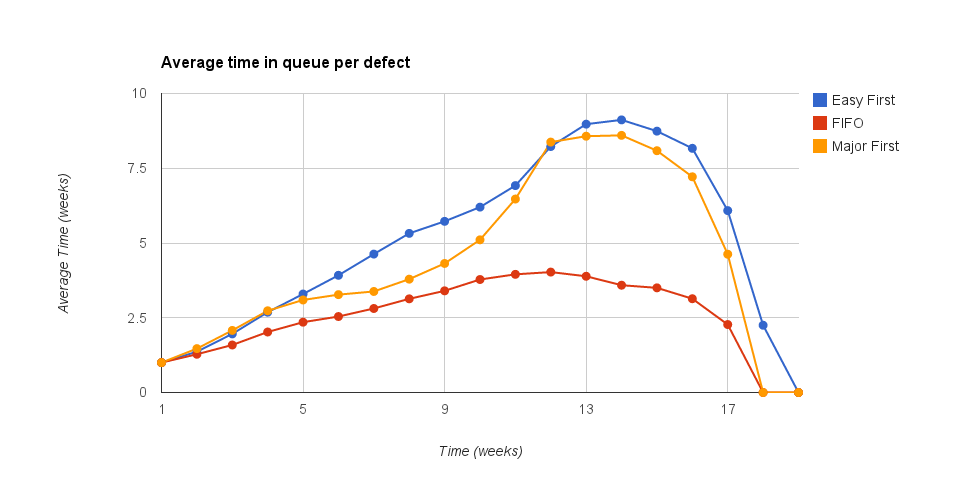
\includegraphics[scale=0.45]{graphs/avgQueueTime.png}
	\caption{The average time a defect spends in the queue is of course actually minimsed by the FIFO
strategy, since it endeavours to fix earliest defects as soon as possible, without any other
reorderings.} 
	\label{avgqtime}
\end{figure}

This does not really go against our logic --- it is a proof that at least without resource
reallocations the system behaves as we expect.\\
\\
Finally, we showcase the defect ratios for find-versus-fixed.

\pagebreak

\begin{figure}[ht!]
	\centering
	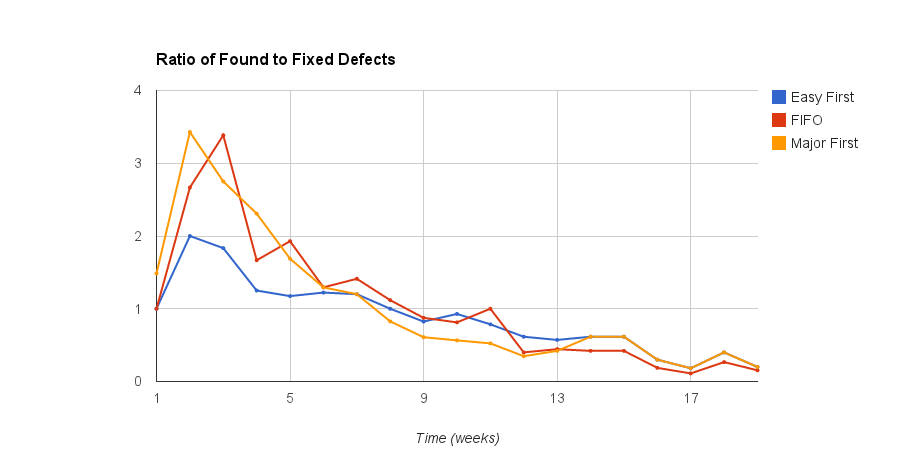
\includegraphics[scale=0.5]{graphs/RatioFF.png}
	\caption{Here, we notice that the optimal choice is to use the easy strategy again, which is a
reflection of our previous metrics and how the easy strategy fixes the highest number of defects.} 
	\label{ratioff}
\end{figure}

As expected, Figure \ref{ratioff} shows that the easy strategy is the optimal for performance using
this metric.\\
\\
We have tabulated our results in a coarse approximation of how ``good" each strategy performed for
each metric.

\begin{table}[ht!]
	\centering
	\begin{tabular}{|c|c|c|}
	\hline
	{\bf Metric} & {\bf Optimal} & {\bf Sub-optimal, but close?} \\ \hline
	{\em Queue Severity} & Major First & N/A \\ \hline
	{\em Mean time in queue per major defect} & Major First & N/A\\ \hline
	{\em Ratio of Major defects found-to-fixed} & Major First & Easy-first \\ \hline
	Queue Size & Easy First & N/A \\ \hline
	Time in Queue & FIFO & Not that close, but Major First \\ \hline
	Ratio of defects found-to-fixed & Easy First & Major First\\ \hline
	\end{tabular}
	\caption{A summary of our strategies and their performances with different metrics.
External metrics are italicised.
It seems clear that the strategy which externally appears best is major first, whilst internally
easy-first appears best.}
	\label{summary}
\end{table}

\subsubsection{External pressure leading to resource change}

Now, we suppose that if the queue severity is too high (that is, existing defects are negatively
affecting the client too much) then a resource reallocation is required.
It is not a very intelligent decision making system, in that it simply reallocates the resources for
the week and keeps them allocated as such until the queue severity is low again.
We can compare it to a bang-bang controller in embedded systems and robotics.\\
\\
Before we begin, we will note an experimental error that we came across but were too late in fixing.
During our measurements for estimating the number of defects left, the FIFO strategy had some
strange occurrences and started outputting negative estimates.
We could not trace where the error in our methodology is, and we have removed it from our
comparisons for external influences.
We present the initial estimates with FIFO included to show how the results were mangled.

\begin{figure}[ht!]
	\centering
	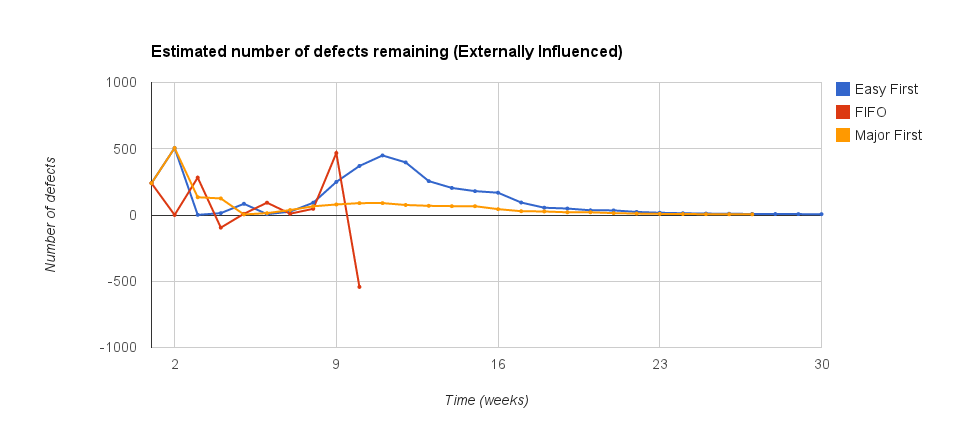
\includegraphics[scale=0.45]{graphs/EstRemDefs_ex.png}
	\caption{Negative estimates for absolute metrics are somewhat confusing.} 
	\label{ex_estremdefs}
\end{figure}

\pagebreak

Similarly with the results for Estimated Remaining Major defects.

\begin{figure}[ht!]
	\centering
	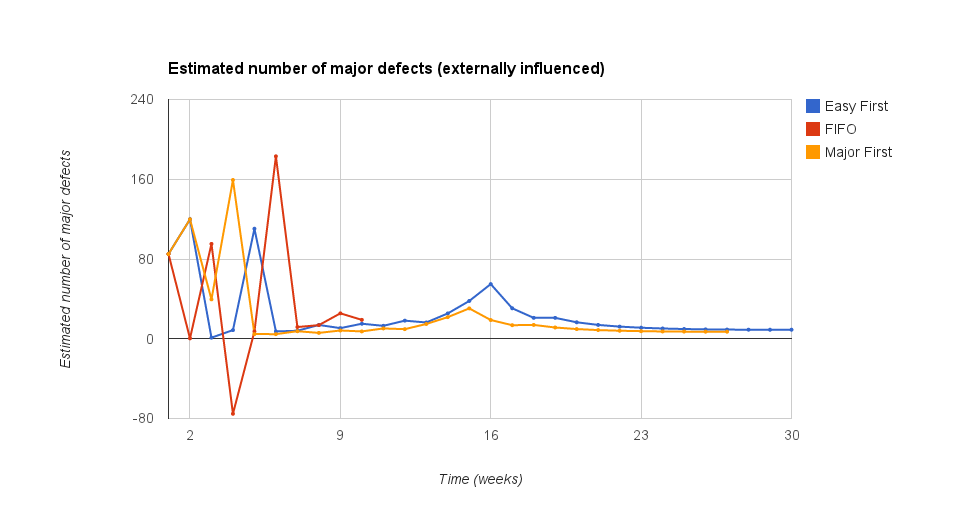
\includegraphics[scale=0.45]{graphs/EstRemMajDef_ex.png}
	\caption{We could not trace this experimental error and thus decided to not use the FIFO strategy
for this measurement.} 
	\label{ex_estremmajdef}
\end{figure}

Other oddities include that the strategies now continue for longer, attempting to finish and
continue fixing defects even though there is nothing new being found or fixed.
They also changed when they stopped due to reassigning the software engineers to testing and fixing
at different times.
Sensible project managers would have stopped testing by now; we have left this in here to showcase
how our system worked.

\pagebreak

We first begin by looking at the external metrics.
As noted earlier, this governs what the client (might!) be thinking about our project and the strategies we have used.

\begin{figure}[ht!]
	\centering
	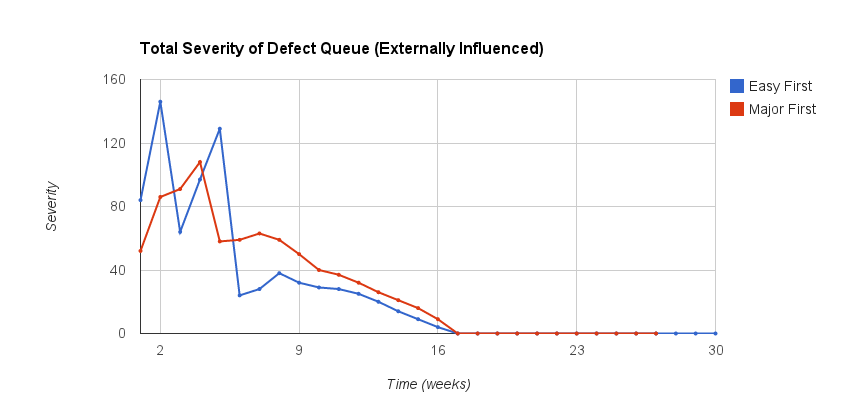
\includegraphics[scale=0.5]{graphs/QueueImpact_ex.png}
	\caption{Notice the large oscillations due to resource reallocation.} 
	\label{ex_qimpact}
\end{figure}

It is interesting that choosing a ``better" strategy is difficult here.
The steadier strategy is to choose major defects first, but the strategy that it is beaten by is to
choose the easier defects first.
The strategy allows spikes in severity levels, however.
We will tentatively claim that here, the easy first strategy is better, despite the sudden surgest
in queue severity.

\pagebreak

What about the average time of major defects in the queue?

\begin{figure}[ht!]
	\centering
	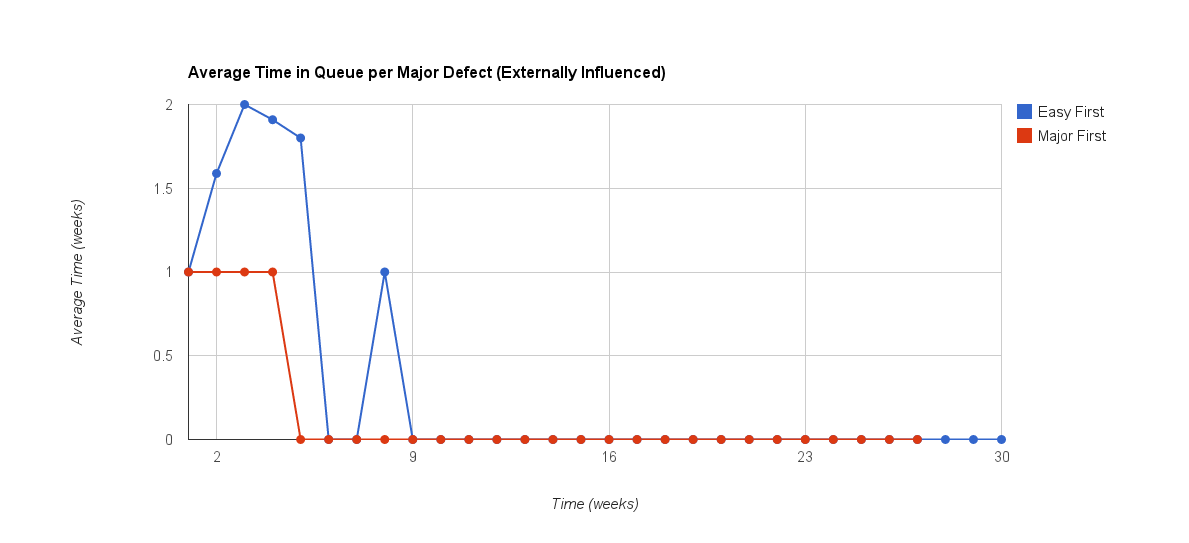
\includegraphics[angle=90,scale=0.4]{graphs/avgMajorQueueTime_ex.png}
	\caption{Overall, high prioritisation of major defects still results in low mean time in queue for
major defects.} 
	\label{ex_avgmajqtime}
\end{figure}

From Figure \ref{ex_avgmajqtime} it is clear that fixing major defects is still the best choice to have a
high performance for average major queue time.

\pagebreak

Next, we briefly examine the find-versus-fixed ratio for major defects.

\begin{figure}[ht!]
	\centering
	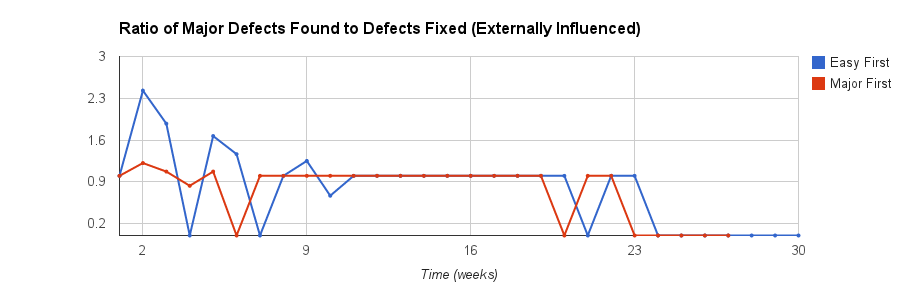
\includegraphics[scale=0.45]{graphs/MajRatioFF_ex.png}
	\caption{Interestingly, very little blowup from the easy strategy --- the resource reallocation is
allowing it to stop the ratio of fixed-found defects from escalating and instead causes it to
oscillate.} 
	\label{ex_majratioff}
\end{figure}

Again we see that the optimal strategy for this metric is to fix major defects first.
However, the differences are much smaller and the strategies are many times on par with each other!
This is quite interesting, when comparing Figure \ref{ex_majratioff} to Figure \ref{majratioff}.

\pagebreak

Next, we examine the internal metrics.
How big is our defect queue size?
Are the resource reallocations causing it to smoothen out a lot?

\begin{figure}[ht!]
	\centering
	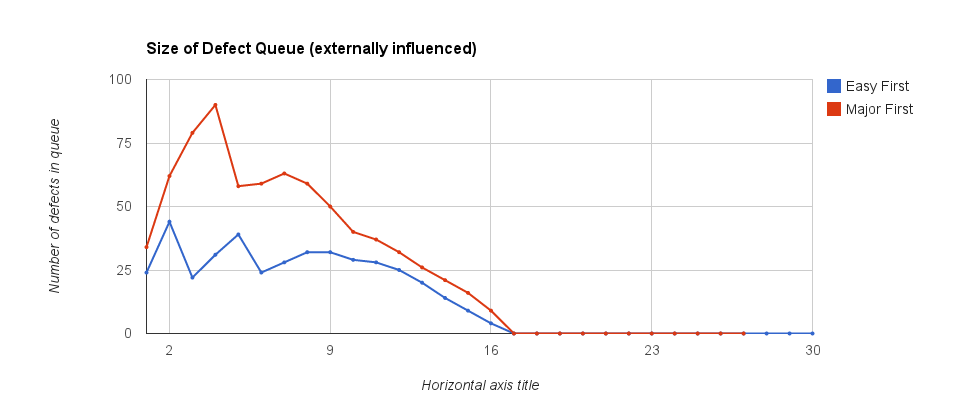
\includegraphics[scale=0.45]{graphs/QueueSz_ex.png}
	\caption{The size of our defects-to-fix queue. Again the optimal choice is to use the easy
strategy.} 
	\label{ex_qsz}
\end{figure}

Figure \ref{ex_qsz} gives what would be the self-evident result --- that prioritising easy defects
yields the best rewards.
There is not as much change here, since severity minimisation does not necessarily entail defect
queue minimisation, as this result shows.\\
\\
We would expect something similar to occur when looking at the average time a defect spends in a
queue, wouldn't we?

\pagebreak

\begin{figure}[ht!]
	\centering
	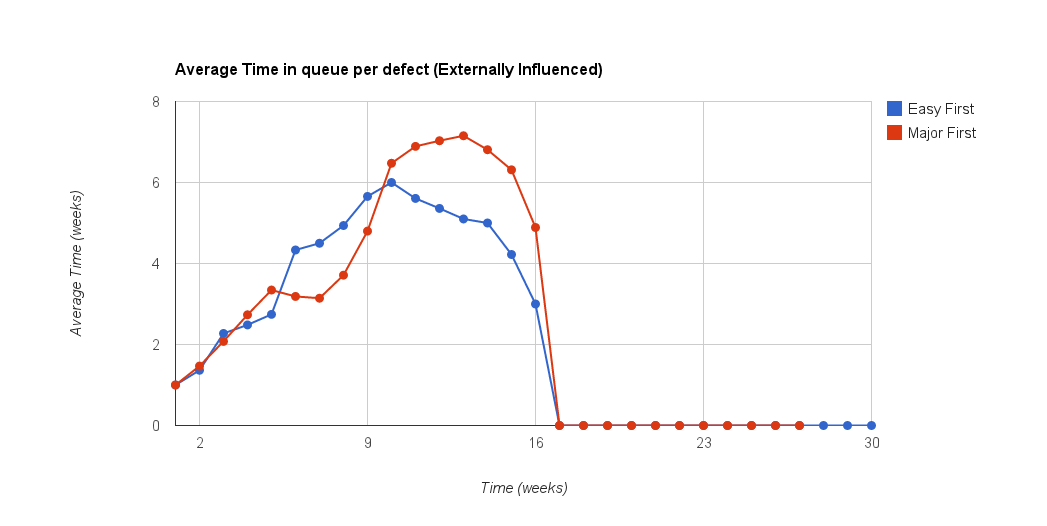
\includegraphics[scale=0.45]{graphs/avgQueueTime_ex.png}
	\caption{This metric seems to be optimally minimised by the easy strategy but fixing major defects
first is very, very close.} 
	\label{ex_avgqtime}
\end{figure}

This seems to be an oscillating reflection of the original results found in Figure
\ref{ex_avgqtime}.
Not a major change, which is a shame as it would have been interesting to see how the previously
optimal strategy, FIFO was affected by resource reallocations.\\
\\
Finally, we showcase the defect ratios for find-versus-fixed.

\pagebreak

\begin{figure}[ht!]
	\centering
	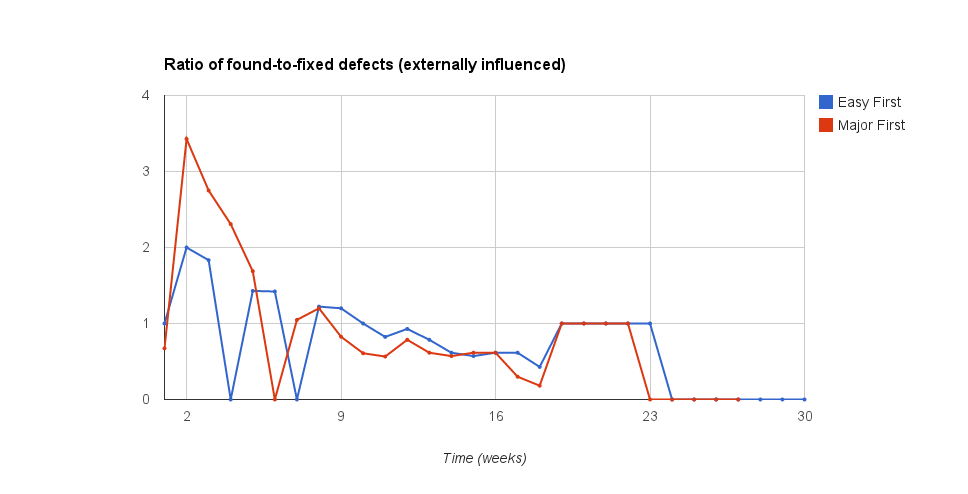
\includegraphics[scale=0.45]{graphs/RatioFF_ex.png}
	\caption{Here, we notice that the optimal choice is to now use the major strategy.} 
	\label{ex_ratioff}
\end{figure}

Figure \ref{ex_ratioff} shows an interesting result! Although major begins poorly, the resource
reallocations have it consistently beating the easy strategy for a large part of the process.
We would tentatively say that major is a better strategy, but that the easy-defects-first strategy
is almost as optimal.\\
\\
We have tabulated our results in a coarse approximation of how ``good" each strategy performed for
each metric.

\begin{table}[ht!]
	\centering
	\begin{tabular}{|c|c|c|}
	\hline
	{\bf Metric} & {\bf Optimal} & {\bf Sub-optimal, but close?} \\ \hline
	{\em Queue Severity} & Easy First & Major First \\ \hline
	{\em Mean time in queue per major defect} & Major First & N/A\\ \hline
	{\em Ratio of Major defects found-to-fixed} & Major First & Easy-first \\ \hline
	Queue Size & Easy First & N/A \\ \hline
	Time in Queue & Easy First & Major First \\ \hline
	Ratio of defects found-to-fixed & Major First & Easy First\\ \hline
	\end{tabular}
	\caption{A summary of our strategies and their performances with different metrics when external
pressure is applied.
External metrics are italicised.
Interestingly, the differences between the strategies have been minimised and they seem to perform
similarly relative to each other.
They all were much more jagged and oscillated a lot due to the sudden resource reallocations.}
	\label{summaryex}
\end{table}

\subsubsection{Internal pressure leading to resource change}

Now, we suppose that if the queue size is too high (that is, there are too many existing defects) then a resource reallocation is required.
It is not a very intelligent decision making system, in that it simply reallocates the resources for
the week and keeps them allocated as such until the queue severity is low again.
Also, the reallocation involves all testers becoming fixers for the week.
We can compare it to a bang-bang controller in embedded systems and robotics.\\
\\
Firstly, we present the estimates of remaining defects.

\begin{figure}[ht!]
	\centering
	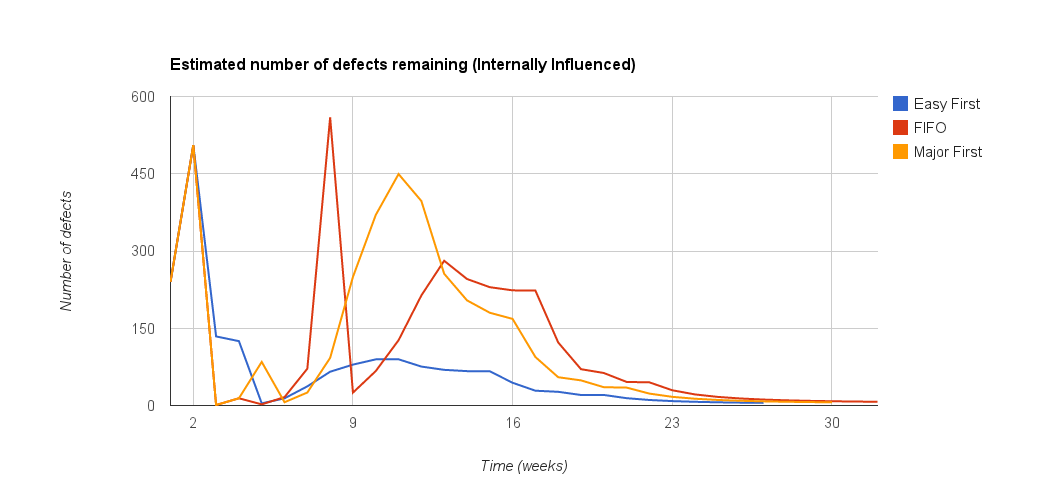
\includegraphics[scale=0.45]{graphs/EstRemDefs_in.png}
	\caption{We note that the resource reallocations again caused high oscillations, except for the
easy strategy.} 
	\label{in_estremdefs}
\end{figure}

Interestingly, the easy strategy appeared to not undergo many resource reallocations or
oscillations.

\pagebreak

A similar result occurs with estimates of remaining major defects.

\begin{figure}[ht!]
	\centering
	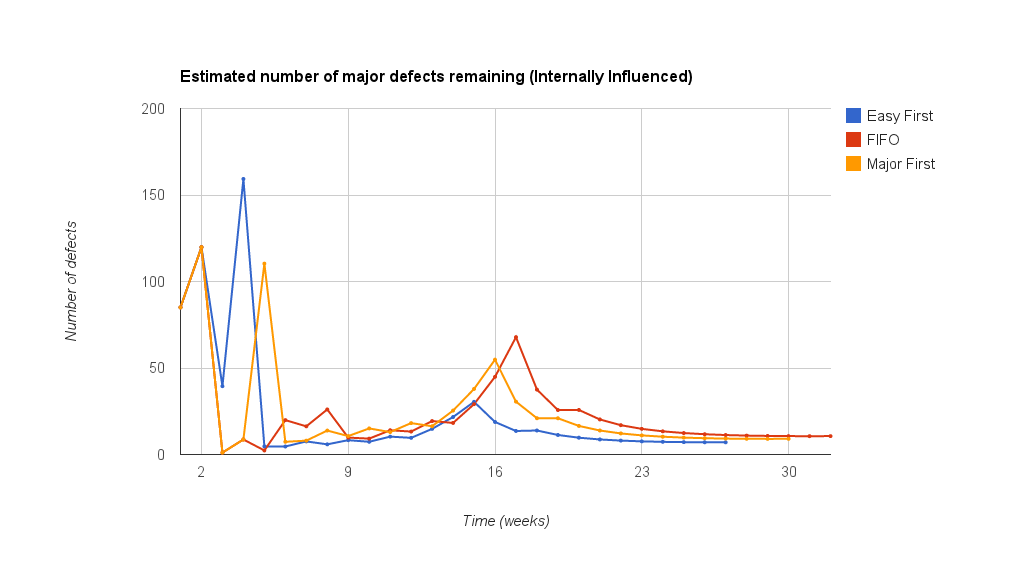
\includegraphics[scale=0.45]{graphs/EstRemMajDef_in.png}
	\caption{This time, it also appears that the FIFO strategy does not have a huge amount of
oscillation.} 
	\label{in_estremmajdef}
\end{figure}

We still have the oddity that the strategies now continue for longer, attempting to finish and
continue fixing defects even though there is nothing new being found or fixed.
Strategies again have different stopping times due to changes for when they stopped due to reassigning the software engineers to testing and fixing
at different times.
Again, a sensible project manager would have stopped testing by now.

\pagebreak

We first begin by looking at the external metrics.
As noted earlier, this governs what the client (might!) be thinking about our project and the strategies we have used.

\begin{figure}[ht!]
	\centering
	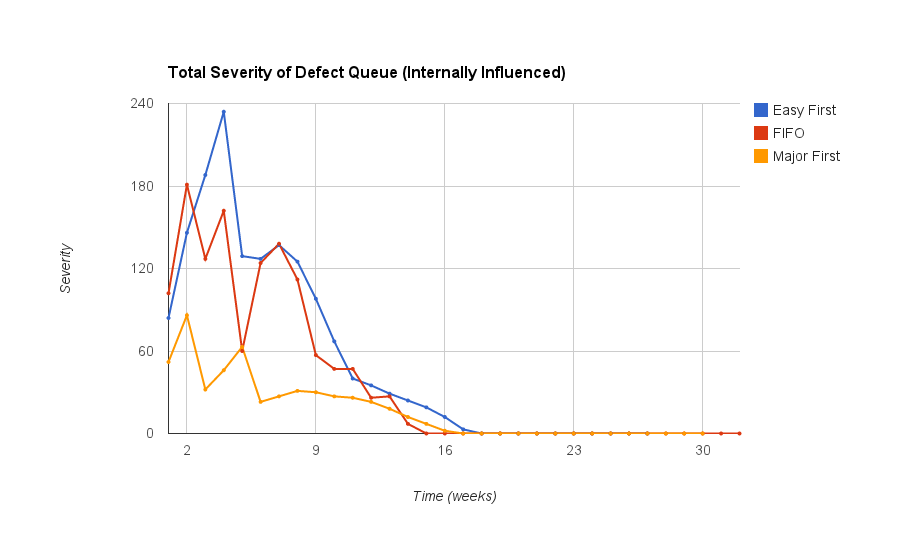
\includegraphics[scale=0.5]{graphs/QueueImpact_in.png}
	\caption{The major-fixes first strategy seems improved by the resource reallocation.}
	\label{in_qimpact}
\end{figure}

It is clear that the major-fixes first strategy is again the best strategy.

\pagebreak

What about the average time of major defects in the queue?

\begin{figure}[ht!]
	\centering
	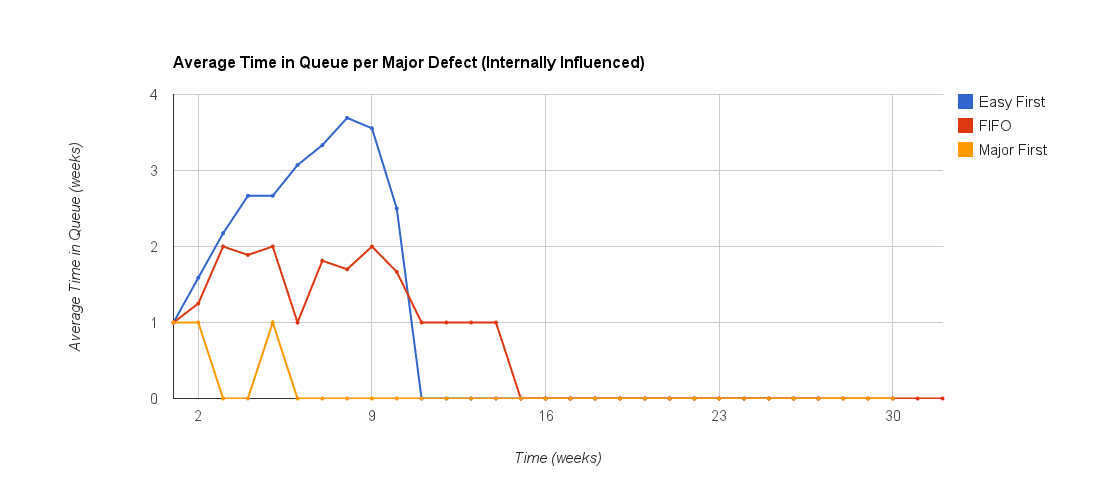
\includegraphics[angle=90,scale=0.4]{graphs/avgMajorQueueTime_in.png}
	\caption{Overall, high prioritisation of major defects still results in low mean time in queue for
major defects.} 
	\label{in_avgmajqtime}
\end{figure}

From Figure \ref{in_avgmajqtime} it is clear that fixing major defects is still the best choice to have a
high performance for average major queue time.

\pagebreak

Next, we briefly examine the find-versus-fixed ratio for major defects.

\begin{figure}[ht!]
	\centering
	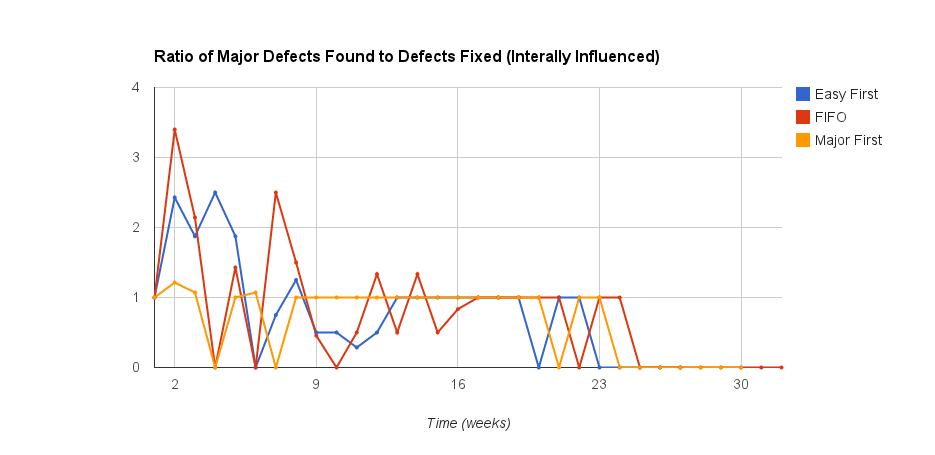
\includegraphics[scale=0.45]{graphs/MajRatioFF_in.png}
	\caption{Interestingly, very little blowup from the easy strategy --- the resource reallocation is
allowing it to stop the ratio of fixed-found defects from escalating and instead causes it to
oscillate.} 
	\label{in_majratioff}
\end{figure}

Again we see that the optimal strategy for this metric is to fix major defects first.
However, the differences are much smaller and the strategies are many times on par with each other!
This is quite interesting, when comparing Figure \ref{in_majratioff} to Figures \ref{majratioff} and
\ref{ex_majratioff}.

\pagebreak

Next, we examine the internal metrics.
How big is our defect queue size?
Are the resource reallocations causing it to smoothen out a lot?

\begin{figure}[ht!]
	\centering
	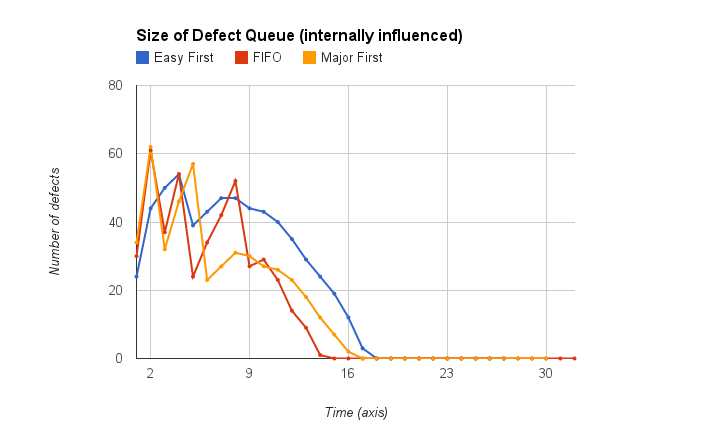
\includegraphics[scale=0.45]{graphs/QueueSz_in.png}
	\caption{The size of our defects-to-fix queue.
An interesting change is that this makes both the FIFO and major-fixes-first strategy better than
the easy-fixes-first strategy.} 
	\label{in_qsz}
\end{figure}

Figure \ref{in_qsz} gives an interesting result --- the resource reallocations have actually
improved the FIFO and major-defects-first strategies.
FIFO is optimal, and major-defects close to being as good in this situation.\\
\\
We would expect something similar to occur when looking at the average time a defect spends in a
queue, wouldn't we?

\pagebreak

\begin{figure}[ht!]
	\centering
	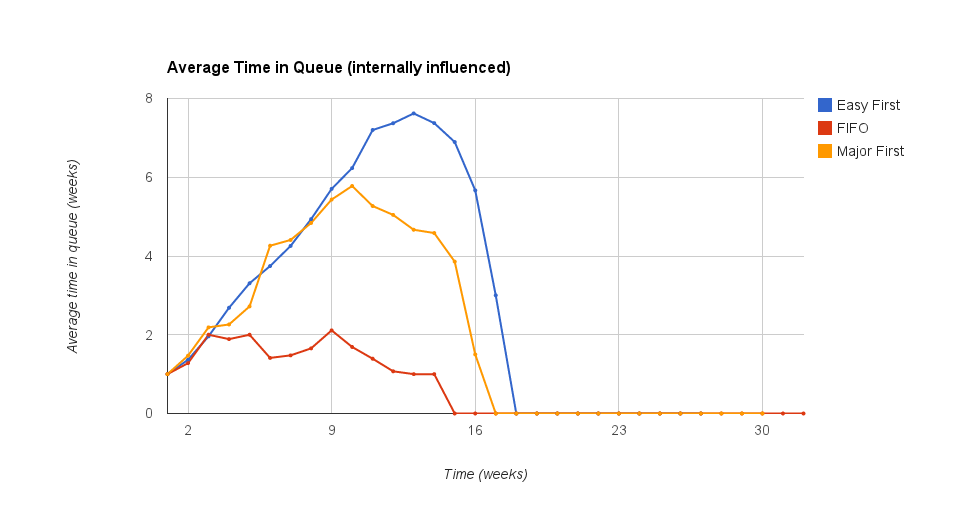
\includegraphics[scale=0.45]{graphs/avgQueueTime_in.png}
	\caption{FIFO is the clear optimal choice here. It already was a queue minimiser and with the
resource reallocation it even better.} 
	\label{in_avgqtime}
\end{figure}

FIFO is clearly the optimal choice again --- adding the resource reallocation has really made it
minimise time in queue.\\
\\
Finally, we showcase the defect ratios for find-versus-fixed.

\pagebreak

\begin{figure}[ht!]
	\centering
	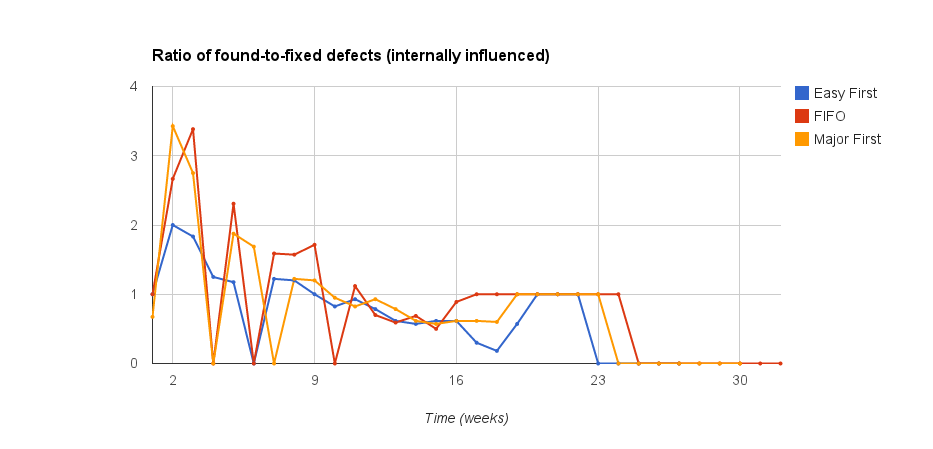
\includegraphics[scale=0.45]{graphs/RatioFF_in.png}
	\caption{The easy-fixes-first is again the best strategy to use in this situation.}
	\label{in_ratioff}
\end{figure}

Surprisingly, there were no changes even after resource reallocations --- the easy-fixes-first was
the best strategy one could use.\\
\\
We have tabulated our results in a coarse approximation of how ``good" each strategy performed for
each metric.

\begin{table}[ht!]
	\centering
	\begin{tabular}{|c|c|c|}
	\hline
	{\bf Metric} & {\bf Optimal} & {\bf Sub-optimal, but close?} \\ \hline
	{\em Queue Severity} & Major First & N/A \\ \hline
	{\em Mean time in queue per major defect} & Major First & N/A\\ \hline
	{\em Ratio of Major defects found-to-fixed} & Major First & Easy-first \\ \hline
	Queue Size & Easy First & N/A \\ \hline
	Time in Queue & FIFO & N/A \\ \hline
	Ratio of defects found-to-fixed & Easy-first & All quite close \\ \hline
	\end{tabular}
	\caption{A summary of our strategies and their performances with different metrics when external
pressure is applied.
External metrics are italicised.
Employing this strategy for resource reallocation (based on queue size) seemed to yield good results, in terms of making
strategies competent against the easy strategy, whilst maintaining properties such as low queue
severity or time of major defect in queue.}
	\label{summaryex}
\end{table}

